\documentclass[12pt]{article}

\usepackage{sbc-template}

\usepackage{graphicx,url}

%\usepackage[brazil]{babel}   
\usepackage[utf8]{inputenc}  

\sloppy

\title{Identifying (deep) fake news communities on multiple social networks}

\author{Thiago Amado Costa\inst{1}, Humberto Torres Marques Neto\inst{1}}


\address{ICEI – Pontifícia Universidade Católica de Minas Gerais (PUC-MG)\\
    Belo Horizonte, Minas Gerais - Brasil 
    \email{thiago.amado@sga.pucminas.br, humberto@sga.pucminas.br}
}

\begin{document}

\maketitle

\begin{abstract}
	The misuse of Deepfakes and the rise of Fake News have become a significant challenge in the
	era of social media, posing serious threats to the credibility of information shared online.
	Additionally, individuals and groups can become targets of these malicious actions, creating
	communities that believe and share news of the same malicious sources.
	This problem is not exclusive to a single social media platform, which highlights the urgent
	need for robust fact-checking mechanisms, as well as solutions to identify these specific
	communities, that will help create a safer online environment.
\end{abstract}

\section{Introduction}
% >> Descrição de motivações
% >> Problema escolhido e objetivos

Fake News and Deepfakes are one of the biggest challenges in today's social media, threatening the
credibility of information shared online.
Fake News is defined as incorrect or misleading information fabricated to mimic the structure of
the news media, but without the process of ensuring accuracy and credibility (\cite{lazer2018science}),
and Deepfake is a form of multimedia manipulation that leverages advanced machine learning and artificial
intelligence techniques to manipulate or generate visual and audio content, with a high capacity to deceive
viewers (\cite{KIETZMANN2020135}).

This phenomenon poses serious threats to today's social media, as it spreads faster and more broadly
than credible information (\cite{doi:10.1126/science.aap9559}), and Deepfakes are becoming more
accessible and believable (\cite{KIETZMANN2020135}). This reinforces the importance of further
research on this topic.
Hence, the primary objectives of this study are to analyze various methodologies for detecting
Fake News and Deepfakes, as well as to examine and identify the communities associated with them.

\section{Related Work}

Identifying and mitigating the spread of fake news has become a pressing concern in recent years,
as the proliferation of social media platforms has enabled the rapid dissemination of
misinformation.
In this section, we review existing research that focuses on detecting fake news,
as well as  communities across multiple social networks.

\subsection{Fake News}

The spread of fake news has become a major concern, impacting public opinion and civil debate.
To combat this, researchers from many fields are developing methods to identify false information.
This section explores key studies and approaches used in detecting fake news.

\cite{Ruchansky_2017} combines text, response, and source characteristics of news articles to approach
the fake news dectection.
Unlike existing solutions that focus on individual aspects, the CSI model integrates these three
key features using deep neural networks to automatically select important information and capture
temporal dependencies in user engagement. By providing insights on both articles and users,
CSI offers a more comprehensive understanding of fake news propagation. Experimental results on
real-world datasets demonstrate that the CSI model achieves higher classification accuracy compared
to previous methods, while also requiring fewer parameters and training efforts.
This highlights the effectiveness of the CSI model in accurately detecting fake
news and addressing the challenges associated with automated fake news detection.

\cite{DeepFakE} introduces a new model called DeepFakE for improving fake news detection by combining news content and social context.
The approach combines news content and social context-based features in a tensor,
resulting in a higher-order decision boundary and achieving state-of-the-art results for fake news detection.
The article shows the significance of examining the social context for improving fake news detection.
It emphasizes the role of user social engagements and echo chambers in the dissemination of fake news.
Echo chambers, which are groups of like-minded individuals, play a vital role in the spread of fake news as
they tend to share stories that align with their beliefs.
The article suggests that utilizing echo chambers to obtain user-related and community-related
information from news articles can enhance fake news detection.

\cite{chandra2020graphbased} discusses the use of different baselines for fake news detection, including text-based,
majority sharing, and social baselines. It compares the article sharing behavior of users in two datasets,
GossipCop and HealthStory, highlighting differences in user characteristics and community graph structures.
The study shows that GNNs are more effective in detecting fake articles in GossipCop due to richer community-level features,
while struggling in HealthStory due to limited user representations and mixed article sharing patterns.
The proposed graph-based approach outperforms text-based models, emphasizing the importance of community-based modeling in fake news detection.

\cite{shu2018news} explores the role of social context in detecting fake news, proposing a TriFN framework that considers the tri-relationship
among publishers, news pieces, and users for classification. It highlights that social context features are more effective
than news content features in predicting fake news, with user-based, post-based, and network-based features playing crucial roles.
The study demonstrates that the TriFN approach significantly outperforms other baseline methods for fake news detection,
showcasing the importance of considering social context in combating fake news.


\subsection{Social Media Communities}

Community detection has garnered significant attention across various disciplines due to its applications
in understanding the structure and dynamics of complex systems.
Over the years, researchers have proposed numerous algorithms and methods to identify cohesive groups within networks.
In this section, we provide an overview of key works in the field.

\cite{Raghavan_2007} proposes a new algorithm for efficiently detecting communities in large networks.
The algorithm leverages a label propagation approach where nodes iteratively adopt the most
common label among their neighbors. This simple strategy facilitates the formation of communities without
requiring prior knowledge about their structure or size. The effectiveness of the algorithm is demonstrated
on well-established benchmarks, achieving high accuracy. Moreover, the algorithm boasts a near-linear time complexity,
making it significantly faster than existing methods. Furthermore, it bypasses the need for complex function
optimization or parameter tuning, offering a more straightforward and
computationally efficient approach to community detection in large-scale networks.

\cite{ZHANG2016133} proposes a parallel label propagation algorithm to identify communities within social networks.
It tackles shortcomings of the traditional label propagation method.
The new algorithm incorporates grey relational analysis during label updates, leading to less randomness in label selection.
Additionally, it optimizes the parallel computation steps. Experiments on various social networks, both simulated and real-world, demonstrate
that this approach is scalable and delivers high accuracy in identifying communities

\cite{Chunaev_2020} dives into the challenge of uncovering communities within social networks, highlighting the importance of considering both
the network's structure (connections between users) and the attributes of individual users (interests, demographics).  A key point
addressed is the current lack of knowledge on how these two aspects influence the accuracy of community detection.
To shed light on this, the article provides a classification system for different community detection methods based on how they
integrate network structure and node attributes. This classification goes beyond just naming categories, offering technical details and
insights into how these methods perform. The article explores various approaches like those based on metaheuristics, probabilistic models,
and reaching consensus among different detection strategies.

\cite{ZHAO2021358} introduces a community detection algorithm (CDEP) designed for massive social networks.
The algorithm leverages graph compression techniques to efficiently identify communities within these complex structures.
Notably, CDEP outshines several existing cutting-edge algorithms in terms of both effectiveness and efficiency.
When tested on various social networks, CDEP consistently revealed community structures that
closely matched real-world groupings. Moreover, it achieved optimal modularity scores, a key metric for
community detection quality.  Furthermore, CDEP stands out as the only method capable of tackling large-scale
networks within a practical time frame, demonstrating its exceptional scalability.

\cite{Cinelli_2021} investigates how social media platforms like Facebook, Twitter, and Reddit contribute to the echo chamber effect.
The researchers define ways to measure echo chambers by examining how users with similar viewpoints connect and share information
(homophily in interaction networks) and how information slants towards reinforcing existing beliefs (bias in information diffusion).
They also establish methods for pinpointing user attitudes on specific topics within these platforms.
By comparing information flow across different social media, the study reveals how content
tends to spread more readily among users who already share similar perspectives.

In \cite{Diaz_2023}, social media is portrayed as a breeding ground for disinformation that thrives on identity politics.
Actors behind the spread of disinformation weaponize rhetoric to manipulate grievances and group affiliation.
This manipulation isn't passive; consumers actively engage in arguments, promoting narratives that challenge established facts.
The article highlights the echo chamber effect as a culprit in solidifying these viewpoints.
Through constant debate within closed communities, arguments become ingrained in personal identities.
The example of Flat Earthers who leverage biblical interpretations to justify their beliefs exemplifies this phenomenon,
where they position themselves as defenders of a purer form of Christianity.

\section{Methodology}

This study uses a combination of news content and social context to detect fake news in its early stages, 
by using the FakeNewsNet data repository proposed by \cite{shu2019fakenewsnet}, 
that currently contains two different datasets with specific news content, social context and
spaciotemporal information, and a version of the User Preference-aware FakeNews Detection (UPFD) framework
proposed by \cite{dou2021user}.  


\subsection{FakeNewsNet Datasets}

The FakeNewsNet dataset is a comprehensive resource designed to aid detection and study of fake news. 
It offers  diverse features that are essential for analysis, including news content, social context, and spatiotemporal information. 

FakeNewsNet includes datasets from two different sources, Polifact and Gossipcop.
One of the significant advantages of FakeNewsNet is its multi-dimensional data, 
which is instrumental for studying early fake news detection, its evolution, and potential mitigation strategies. 

FakeNewsNet can be used for many different research applications, 
such as the study and classification of FakeNews in its early stages by using the social context and spatiotemporal informations.
Another possible application is the identification of malicious actors that play a powerfull role in the spreading of 
Fake News. The FakeNewsNet can also be expanded, by adding support in different languages and different social media platforms.

\subsection{UPFD Framework}

\begin{figure*}
    \centering
    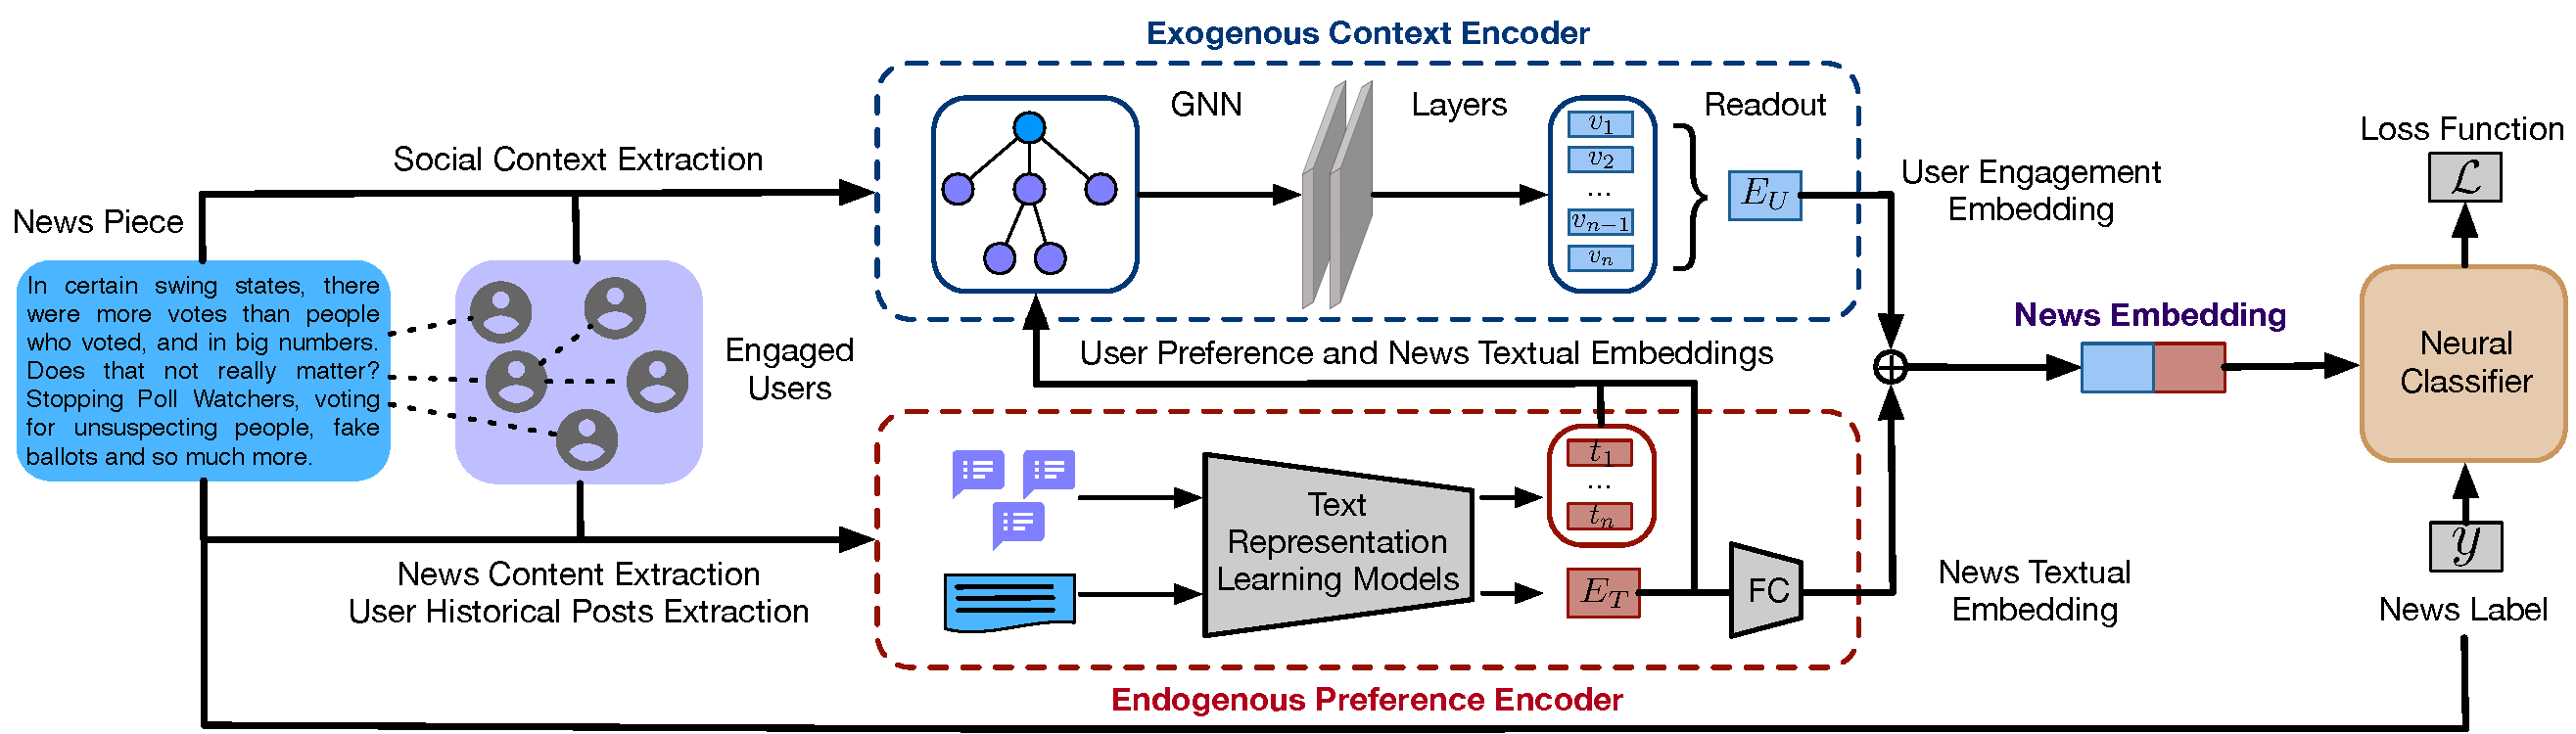
\includegraphics[width=\textwidth]{upfd_framework.pdf}
    \caption{User Preference-aware FakeNews Detection Framework}
    \label{fig:upfd_framework}
\end{figure*}

The User Preference-aware FakeNews Detection framework extracts the 
news textual content and the social context from the datasets to build two Encoders. 

First, the Endogenous Encoder (or the News Textual Encoder) uses pretrained text representation techniques 
to generate the embedding of the news textual information and of historical posts of users who engaged with the news.

The Exogenous Encoder (or the User Engagement Encoder) builds a news propagation graph 
where the root node is the news and the other nodes represent users who reposted the news.
Then, it uses a GNN to fuse the user features with this news propagation path, 
by adding the news textual embedding and user preference embedding as node features, 
to learn the node embeddings. 
By applying a readout function that makes the mean pooling over all node embeddings, 
the News Propagation Graph embedding is obtained.

Finally, a concatenation is made between the News Textual Embedding and the User Engagement Embedding
to create the final News Embedding, that is fed into a Multi-Layer Perceptron with two outputs, representing
real news and fake news probabilities. 
The model training uses a Binary Cross-entropy loss and is updated with Stochastic Gradient Descent (SGD) Optimization.

This framework is illustrated in Figure~\ref{fig:upfd_framework}. 

\subsection{UPFD for Early Detection}

Early detection of fake news is crucial because as the dissemination of fake news increases, 
it becomes increasingly challenging to mitigate its effects. It is also important to consider that
Fake News spreads wider and faster than Real News, as shown by \cite{doi:10.1126/science.aap9559}.

The original User Preference-aware FakeNews Detection framework is used 
considering the entire news propagation path. 
To use it for early detection, the propagation path is clipped to consider only
the first 100 reposts of a given news, and only 20 historical posts of a given user who reposted, 
instead of the original 200. 
User commentaries on the original news post are also considered.
A time limit is also set, to consider only the first hour of spreading.
% The sturcture of the propagation graph is also slightly changed, to be a Time-based news cascade that
% allows a measure of real-time heat (the number of users posting/reposting the news at a given time t), 
% as explained by \cite{Zhou_2020}.


\section{Expected Results}

The objective is to determine whether user preferences and social context can play a 
significant role in identifying fake news in its early stages, 
when the propagation graph is smaller and fewer users have interacted with the news.

As was shown by \cite{dou2021user}, the proposed framework achieved state-of-the-art results
with the FakeNewsNet dataset, with the authors attributing this success to the 
inclusion of user historical posts as part of the social context. 
Given this, incorporating user preferences is expected to enhance the early detection of fake news, 
particularly when compared to methods that consider only news textual content, 
only social context, or both without user preferences.


\bibliographystyle{sbc}
\bibliography{sbc-template}

\end{document}
